\chapter{Dynamic Programming}

Dynamic Programming is the misleading name given to a general method of solving certain optimization problems.  Chances are if a problem asks you to optimize something and doesn't involve a graph, you'll want to use Dynamic Programming.  As always, there are exceptions  (for example, for problems with small upper bounds on $N$, brute force might actually be the way to go).

Dynamic Programming works on problems that can be represented as a series of sub-states.  We can solve the smallest or base state first, then work up from there building up to the solution.  Since we only calculate each sub-state once, the runtime of dynamic programming solutions is polynomial.
%
A simple and overused example of dynamic programming is calculation of the Fibonacci numbers.  Calculating the Fibonacci numbers recursively has an exponential time complexity $O(\varphi^N)$.  But if use dynamic programming to work from the bottom up calculating $F_2$, then $F_3$, etc, it's clear that this is $O(N)$.
%
\begin{figure}[h]
\begin{center}
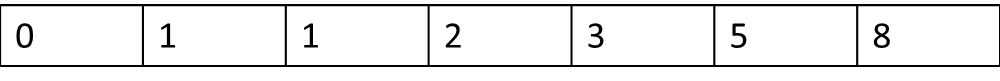
\includegraphics[width=6in]{images/fib-dp.png}
\end{center}
\caption{DP Array for Calculation of the First Few Fibonacci Numbers}
\end{figure}

\section{Knapsack Algorithm}

\begin{figure}[ht]
\begin{center}
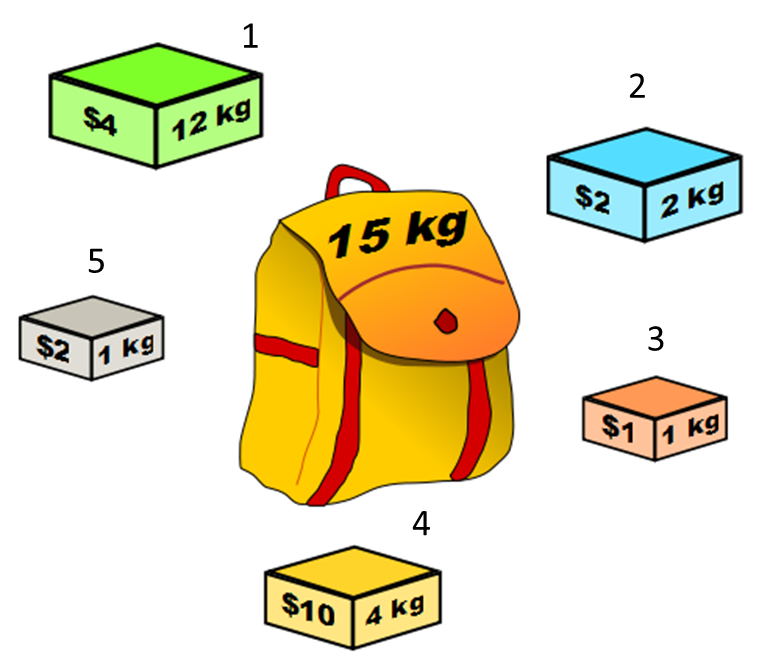
\includegraphics[width=2in]{images/knapsack.png}
\end{center}
\caption{Example Knapsack Problem}
\label{fig:ihatelarry}
\end{figure}

One very common DP problem you'll see on many programming contests is the Knapsack Problem.  There are various forms of the knapsack problem, but the general idea is that you have a ``knapsack'' with some capacity $C$.  You have to fill it with any number of $N$ types of objects of some weight $W[i]$ and value $V[i]$.  Given that the sum of the weights must not exceed $C$, find the maximum value that can be stored in the knapsack.  This specific form of the knapsack problem, where you can have as many or as little of each type of object as you want, is known as the \textbf{Unbounded Integer Knapsack Problem}.
%
By way of example, consider the problem in Figure \ref{fig:ihatelarry}.
%


We know that each of the $N$ types of objects is \textit{in} the knapsack some number of times.  We could go through each type of object and iterate over the number of times it could be in the knapsack, but this is clearly too slow---exponential in $N$.
%
You might think that we can just greedily add the objects with the highest value-to-weight ratio first.  But consider the case $C = 10$ with two types of objects: $\{V_1 = 8, W_1 = 6\}$, $\{V_2 = 5, W_2 = 5\}$.  We would greedily add object $1$, yielding a value of $8$.  However, a cleverer person would add two object $2$s, thus yielding a value of $10$.
%
\subsection{Dynamic Programming Approach}
Suppose instead of finding the maximum value obtainable with $C$ as the capacity, we first found the maximum value for some lower capacity limit $c$.  Finding the maximum value for $c=0$, for example, is trivial (it would be 0, because we can't take any objects).  If we now try $c=1$, we can just find which objects have a weight of $1$ and maximize over their values.  In fact, as we increment $c$, we begin to notice a general pattern.  Let's construct an array \verb=dp[c]= that denotes the max value of a knapsack with capacity $c$.  Then with a bit of thought, it's not hard to realize $dp[c] = \max\limits_{\text{item } j} \left[dp[c-W[j]]+V[j]\right]$, assuming we initialize \verb=dp[1...C]= to $-\infty$.  Take a moment to understand why this works.

This function loops through each item type $j$ and determines which is the most beneficial when added to the bag.  If you choose to add an item of type $j$, the remaining capacity of the knapsack will decrease to $c - W[j]$ while the knapsack's value will increase to $dp[c - W[j]] + V[j]$, which is the sum of item type $j$'s value and the value of a knapsack with the remaining capacity $c - W[j]$.  Then, we simply want the max possible value over all possible item $j$'s to add.
%
\begin{figure}[h]
\begin{center}
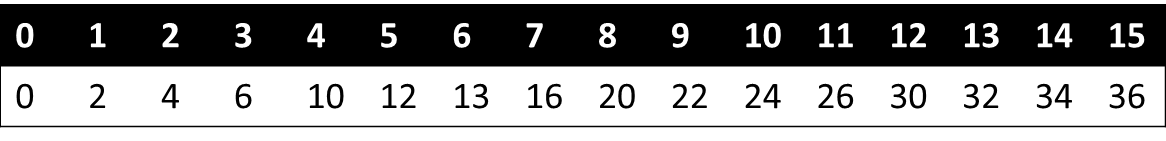
\includegraphics[width=4in]{images/knapsack2.png}
\end{center}
\caption{DP Array - Top Row Represents Capacity, Bottom Row Represents Optimum Value}
\end{figure}

\section{General Strategy}
Now that we've seen an example problem and its dynamic programming solution, is there a general strategy for solving DP problems?  In fact there is.
%
\subsection{Definition of State Variables}
In this step, we essentially need to figure out what the substates are and what variables will change for smaller or larger substates.  We can then construct some array \verb=dp= where accessing \verb=dp[i][j][k]...= returns the desired answer for a given subproblem of those variables $i, j, k, \ldots$.

In the Knapsack example, our substates were the maximum values of the knapsack for smaller capacities.  We could then base the substate on the capacity, creating a one-dimensional \verb=dp= array.  For some substate capacity $i$, \verb=dp[i]= returned the maximum attainable value for that capacity.
%
\subsection{Base Cases}
Having figured out the state variables, we need to determine some base cases, usually at points where the state variables are very small.

In the Knapsack example, we might want to initialize \verb=dp[0]= to $0$ (since a knapsack of $0$ capacity holds $0$ value).  We might also want to initialize the other elements of the array to $-\infty$ so that when we maximize, we make sure not to choose an unattainable capacity.  If we use this method, we have to be careful when choosing the ``maximum'' that \verb=dp[C]= is actually a positive number.  Instead, we might choose the highest element of \verb=dp= that is positive, since this will clearly be the maximum possible value of the knapsack of capacity $C$.
%
\subsection{Transition Functions}
Here's the part that usually requires lots of thought.  We need to figure out the relationship between the elements in our array, and we need to be able to calculate them in a bottom-up approach so that our run time is polynomial.

In the Knapsack example, we chose the function $dp[i] = \max\limits_{\text{item } j} \left[dp[i-W[j]]+V[j]\right]$.  From this, we start at \verb=dp[1]= and continue to \verb=dp[C]=, making sure to traverse in that order (bottom-up).  What made us choose this particular function is that we know we want to consider all the possible ways to get \verb=dp[i]=, and we want to maximize its value.  So for each object $j$, we simply check if the value of that object added to a knapsack of capacity $i-W[j]$ is greater than \verb=dp[i]=.
